%!TEX root = ../thesis.tex
%Adding the above line, with the name of your base .tex file (in this case "thesis.tex") will allow you to compile the whole thesis even when working inside one of the chapter tex files

\chapter{Multi-wavelength Radio Continuum Emission Studies of \\ Dust-free Red Giants} \label{chap:6}

The vast increase in bandwidth coverage of the new VLA now allows possible detections of historically weak or undetectable red giants at multiple radio wavelengths. In this chapter, we present and analyze the most comprehensive set of multi-wavelength thermal radio continuum observations of two standard luminosity class III red giants, Arcturus ($\alpha$ Boo: K2 III) and Aldebaran ($\alpha$ Tau: K5 III), to date. We report the first detections at several wavelengths for each star including a detection at 10 cm (3.0 GHz: S band) for both stars and a 20 cm (1.5 GHz: L band) detection for $\alpha$ Boo. This is the first time single luminosity class III red giants have been detected at these continuum wavelengths. We compare our data with published semi-empirical atmospheric models based on UV data, and spectral indices are used to discuss the possible properties of the stellar atmospheres. Finally, we develop a simple analytical wind model for $\alpha$ Boo based on our new long wavelength flux measurements. This chapter is based on the main results of \cite{ogorman_2013}.

\section{Why Study Red Giants with the VLA?}\label{sec:6.1}
Although studies of wind-scattered UV and optical line profiles have provided clues to the mass-loss rates and radial distribution of the mean and turbulent velocity fields, the thermal structure remains poorly constrained. In the UV, the source function $S_{\nu}$, of electron collisionally excited emission lines is sensitive to electron temperature $T_{\rm{e}}$, (i.e., $S_{\nu} \propto e^{-h\nu /kT_{\rm{e}}}/\sqrt{T_{\rm{e}}}$). Therefore, a localized hot plasma component in a dynamic atmosphere can completely dominate the temporally and spatially averaged emission and hence not reflect the mean radial electron temperature distribution. At radio wavelengths however, the source function is thermal and is just the Rayleigh-Jeans tail of the Planck function, which is linear in electron temperature (i.e., $S_{\nu} = {2kT_{\rm{e}}\nu ^2 /c^2}$). This should give a more appropriate estimate of the mean radial electron temperature. It is this value that controls the atomic level populations and ionization of the mean plasma which is needed to quantify the implied thermal heating supplied to the  wind by the unknown driving source/sources, allowing constraints on potential mass-loss mechanisms to be derived.

In the cm-radio regime the radio opacity $ \kappa _{\lambda}$, strongly increases with wavelength (i.e., $ \kappa _{\lambda} \propto \lambda ^{2.1}$) and so the longer wavelengths sample the extended layers of a stars atmosphere, thus providing us with spatial information about the star's mass outflow region. The VLA is sensitive to over three orders of magnitude in continuum optical depth $\tau _{\lambda}$, ($\tau _{20 \ \rm{cm}}/\tau _{0.7 \ \rm{cm}} \approx 10^3$) and provides an area-averaged sweep through the wind acceleration zone of evolved late-type stars. The thermodynamic properties in this spatial region control the ionization in the far wind because the ionization balance, which also controls the cooling rates, becomes \textit{frozen-in} at large radii due to advection. Furthermore, it is these outer extended regions of the star's atmosphere that contribute to the commonly seen P Cygni line profiles in the UV. In these profiles the line-of-sight absorption caused by the star's wind is superimposed on the blueshifted scattered emission. Thus, centimeter radio continuum observations can provide a test of models based on these UV profiles. 

Despite the importance of radio continuum emission as a tool for studying cool evolved stellar outflows, red giants are feeble emitters at these wavelengths however, and previous observations have provided only a small number of modest signal-to-noise measurements slowly accumulated over three decades. As most of our VLA observations were carried out over just a few days, we have obtained a unique snapshot of the different stellar atmospheric layers sampled at different wavelengths, independent of any long-term variability. 

\section{Radio Maps}\label{sec:6.2}
Apart from $\alpha$ Boo at C band and $\alpha$ Tau at S band, detections were made in every sub-band for the 2011 data. For all other bands, the flux densities of the targets in both sub-bands were found to be the same within their uncertainties so we do not present separate values here. Instead we give the values from the radio maps produced by concatenating the two sub-bands. We present in Table \ref{tab:6.1} the target flux densities extracted from these concatenated radio maps. In each of these maps the flux density from the unresolved target source was calculated by, 1) taking the peak pixel value from the source, 2) manually integrating the flux density around the source, and 3) fitting an elliptical Gaussian model to the source and deriving the integrated flux density using the CASA \textit{imfit} task. Each of these values along with the image rms noise measured from adjacent background regions and fitting error produced by \textit{imfit} are given in Table \ref{tab:6.1} to indicate the quality of each radio map. Both sources are point sources at all frequencies so the peak flux value given in Table \ref{tab:6.1} will also be its total flux density value. For weak detections (i.e., $F_{\nu} \lesssim 5\sigma$) we avoid using the \textit{imfit} task to obtain a flux density estimate, as this may produce biased parameter estimates \citep{taylor_1999}. The flux density values used in the following Sections are the peak values listed in Table \ref{tab:6.1}. We assume absolute flux density scale systematic uncertainties of  3\% at all frequencies \citep{perley_2013}. In the following two sections we briefly discuss the properties of these maps for both targets which are shown in Figure \ref{fig6.2}.



\begin{figure}[htp]
\centering 
\mbox{
		  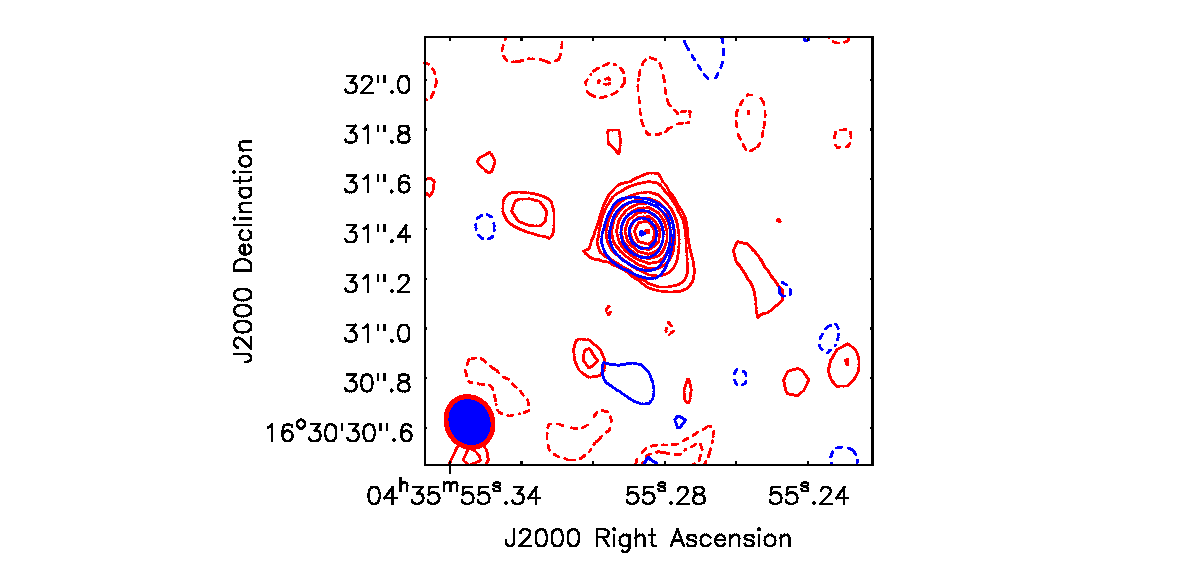
\includegraphics[trim=100pt 50pt 150pt 10pt,clip,width=7.5cm,height=6.0cm]{/home/eamon/thesis/thesis_template/6/atau_q_ka.ps}
          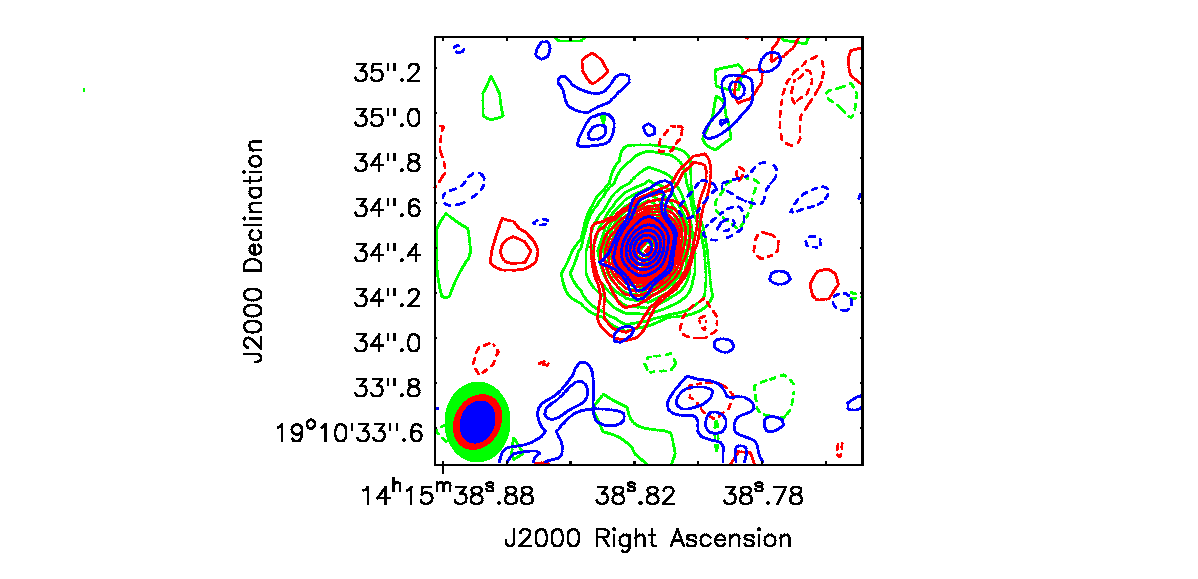
\includegraphics[trim=130pt 50pt 150pt 10pt,clip,width=7.5cm,height=6.0cm]{/home/eamon/thesis/thesis_template/6/aboo_q_ka_k.ps}
          }
\mbox{
          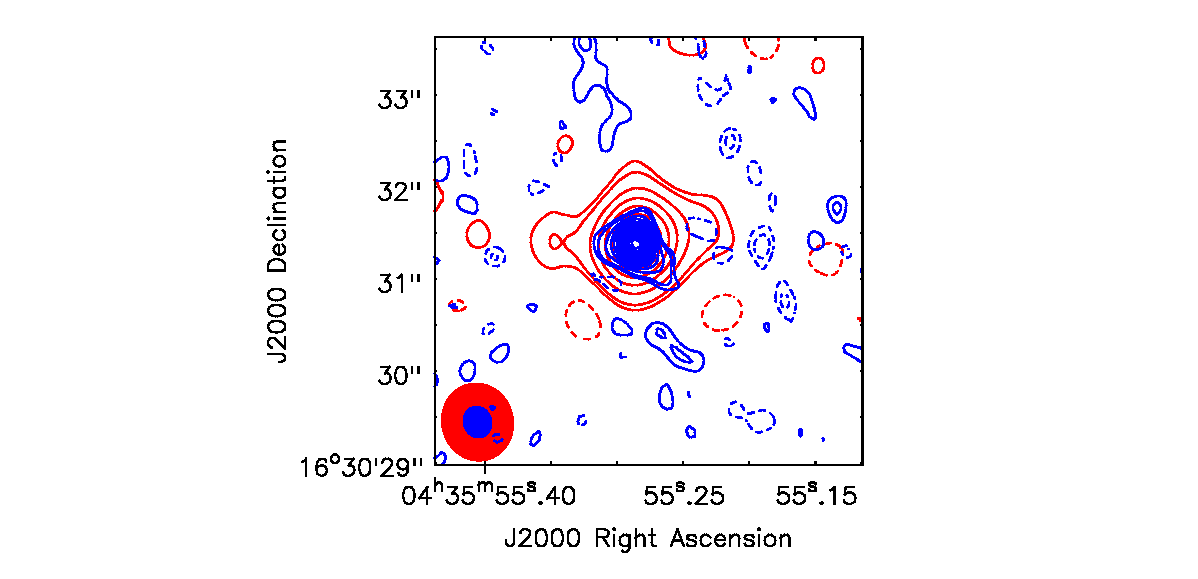
\includegraphics[trim=115pt 50pt 155pt 10pt,clip,width=7.5cm,height=5.8cm]{/home/eamon/thesis/thesis_template/6/atau_x_k.ps}
          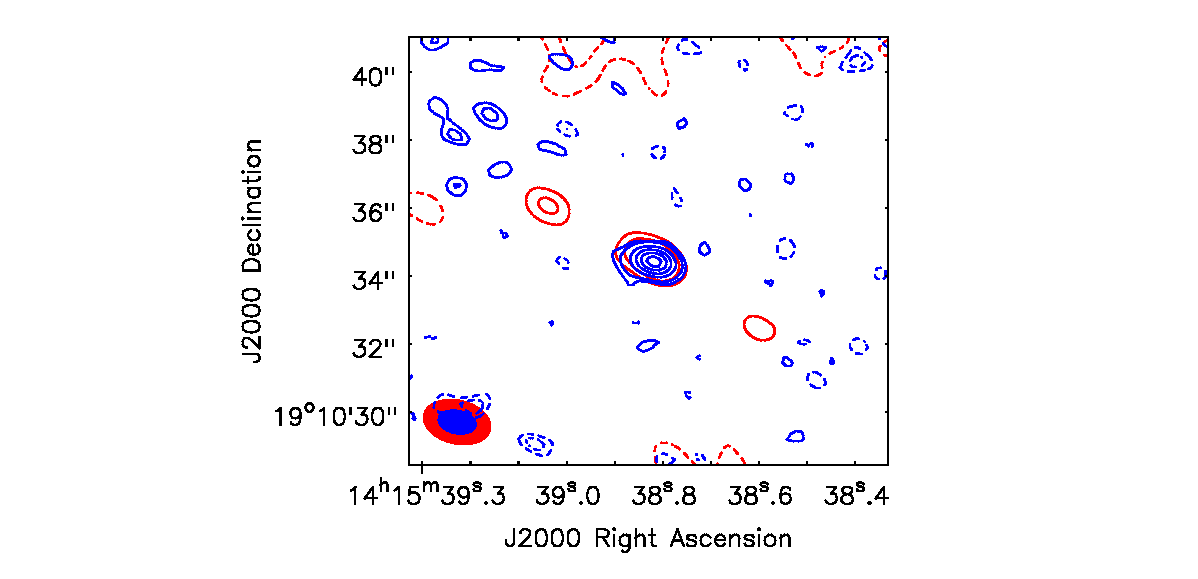
\includegraphics[trim=108pt 50pt 145pt 10pt,clip,width=7.3cm,height=5.8cm]{/home/eamon/thesis/thesis_template/6/aboo_c_x.ps}
          }
\mbox{
          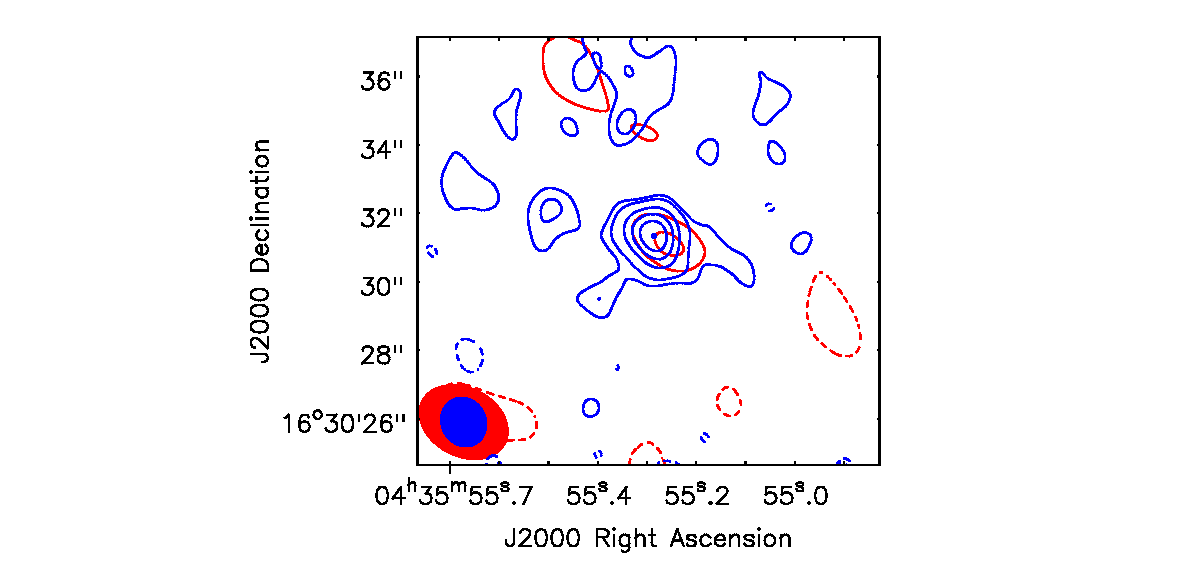
\includegraphics[trim=100pt 10pt 148pt 10pt,clip,width=7.5cm,height=6.4cm]{/home/eamon/thesis/thesis_template/6/atau_c_s.ps}
          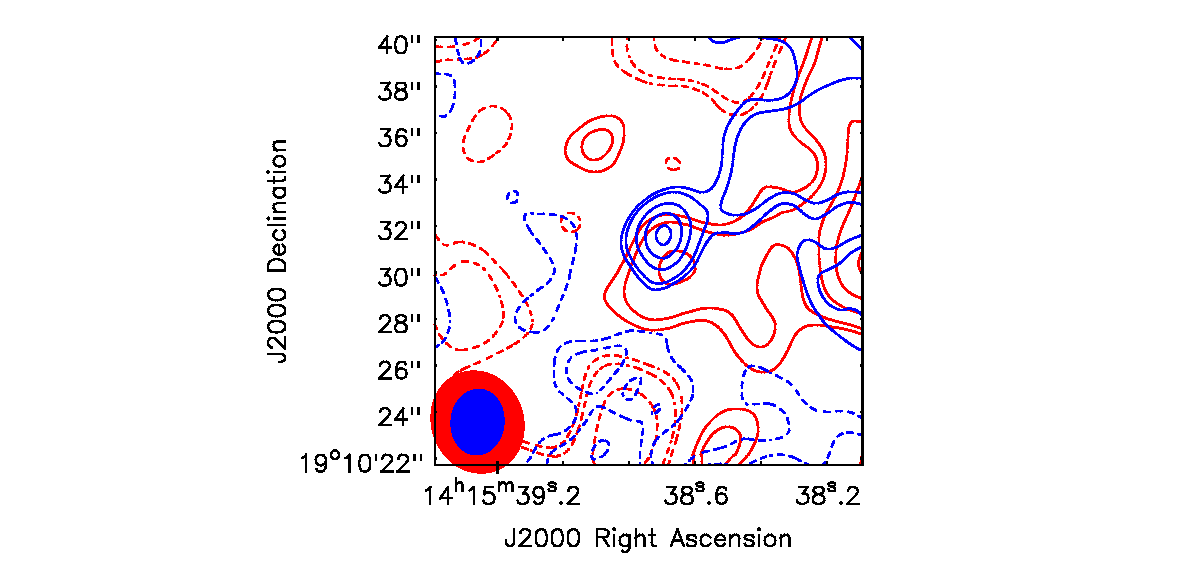
\includegraphics[trim=125pt 10pt 150pt 10pt,clip,width=7.5cm,height=6.4cm]{/home/eamon/thesis/thesis_template/6/aboo_l_s_ddt.ps}
          }
\caption[Final VLA multi-wavelength radio maps of $\alpha$ Boo and $\alpha$ Tau]{Final VLA multi-wavelength radio maps of $\alpha$ Tau and $\alpha$ Boo. \textit{Left column:} Q and Ka band (top), K and X band (middle), C and S band (bottom) maps of $\alpha$ Tau. \textit{Right column:} Q, Ka, and K band (top), X and C band (middle), S and L band (bottom) maps of $\alpha$ Boo. Contour levels are set at $(-6,-3,-2,+2,+3,+6,+9,....)\times \sigma$ where $\sigma$ is the rms noise of each radio map. For $\alpha$ Boo, artifacts from the dirty beam can be seen in the Q band map, while artifacts caused by the serendipitous strong source in the S and L band maps are also present.}
\label{fig6.2}
\end{figure}

\afterpage{\begin{landscape}
\begin{table}[!hb]
\begin{center}
\caption[VLA Flux Densities of $\alpha$ Boo and $\alpha$ Tau]
{VLA Flux Densities of $\alpha$ Boo and $\alpha$ Tau.}
\begin{tabular}{ccccccccc}
\hline
\hline
Star & Band & $\nu ^{\rm{a}}$ & $\lambda$ & Peak $F_{\nu}$ & Integrated  &\textit{Imfit} Integrated & Image rms &\textit{Imfit} Fitting \\
 &  & (GHz) & (cm) & (mJy beam$^{-1}$) & $F_{\nu}$ (mJy)& $F_{\nu}$ (\rm{mJy})&(mJy beam$^{-1}$)&Error (mJy)\\
\hline
\rule{0pt}{2.5ex}$\alpha$ Boo  &Q  &43.28&0.7 &5.94 & 6.09 & 6.42 & 0.30 &  0.26\\
&Ka &33.56&0.9& 4.16 & 4.32 & 4.49 & 0.08 & 0.09 \\
&K  &22.46&1.3& 1.83 & 1.78 & 1.81 & 0.04 & 0.05 \\
&X  &8.46&3.5 & 0.51 & 0.51 & 0.53 & 0.03 & 0.02 \\
&C  &4.90&6.1 & 0.21 & 0.14 & 0.16 & 0.04 & 0.01 \\
&S  &3.15&9.5 & 0.15 & 0.14 & -     & 0.03 & -     \\
&S  &2.87&10.4 & 0.13 & 0.12 & 0.12 & 0.01 & 0.02\\
&L  &1.63&18.4 & 0.07 & 0.07 & -     & 0.01 & -    \\
\hline
\rule{0pt}{2.5ex}$\alpha$ Tau &Q  &43.28 & 0.7&3.67& 3.73 & 4.08 &  0.26& 0.18	\\
&Ka &33.56 & 0.9&2.19& 1.96 & 2.13 &  0.09& 0.07 \\
&K  &22.46 &1.3& 1.86& 1.88 & 2.07 &  0.04& 0.08 \\
&X  &8.46  & 3.5&0.30& 0.29 & 0.28 &  0.01& 0.02 \\
&C  &4.96  & 6.0&0.15& 0.17 & 0.18 &  0.01& 0.01 \\
&S  &3.15  & 9.5&0.06& 0.04 & - &  0.02 & -\\
\hline
\end{tabular}
\label{tab:6.1}
\begin{minipage}{19.cm}
$^{\rm{a}}${\footnotesize Frequency of the final image produced using the multi-frequency synthesis imaging mode within CASA's \textit{clean} task.}
\end{minipage}
\end{center}
\end{table}
\end{landscape}}

\subsection{$\alpha$ Boo Maps}\label{sec:6.2.1}
High S/N detections ($>$19$\sigma$) of $\alpha$ Boo were made at 22.5, 33.6, and 43.3 GHz. Some residuals of the dirty beam remained in the CLEANed maps due to the paucity of uv-coverage in these short high frequency observations (see Figure \ref{fig6.2}, top right panel). At the lower frequencies, it was necessary to image confusing sources, notably a strong radio source located $186\arcsec$ north-west of $\alpha$ Boo. This non-thermal source was reported by \cite{drake_1983} and their flux density of 25 mJy at 4.9 GHz is in close agreement with our measurement of 23.2 mJy at the same frequency. We find the source to have a spectral index $\alpha$ ($F_{\nu} \propto \nu ^{\alpha}$) of -1.4 between 8.5 and 1.6 GHz; its flux density reaches 80.3 mJy at 1.6 GHz.

We detected $\alpha$ Boo at 6$\sigma$ in the lower frequency sub-band of C band, at 4.9 GHz. The noise was slightly higher and the images were poorer quality in the C band higher frequency sub-band, with artifacts exceeding $\pm$200 $\mu$Jy, and we cannot report a detection in this sub-band, so values given in Table \ref{tab:6.1} are taken from the lower frequency sub-band only. We obtain good detections ($>$5$\sigma$) of the star for both epochs at $\sim 3$\,GHz (S band) and the peak flux densities agree within their uncertainties. We can therefore safely assume that the 1.5 GHz (L band) flux density has not changed significantly over that period either, and so can safely be included in any analysis. The map at L band was highly contaminated by the sidelobes of the strong source north-west of $\alpha$ Boo but the star is still detected at the $5\sigma$ level. There is a slight positional offset of $1\arcsec$ between the position of the peak flux density at 1.5 and at 3.0 GHz for the 2012 data, which were taken within 1 day of each other. However, the position uncertainties due to noise and phase uncertainties between the directions of the phase reference source and the target are at least $1\arcsec$, and so we feel that it is highly likely that both detections are of $\alpha$ Boo.

\subsection{$\alpha$ Tau Maps}\label{sec:6.2.2}
The final deconvolved radio maps of $\alpha$ Tau were of excellent quality with the rms noise reaching the predicted noise levels in many cases. The target field at all frequencies was free from strong serendipitous radio sources and thus the final images were free of the sidelobe contamination that were present in the low frequency $\alpha$ Boo images. $\alpha$ Tau was the only source in the high frequency maps while the brightest source in the low frequency maps was located $106\arcsec$ north north-east of $\alpha$ Tau and had flux densities of 0.85, 1.35, and 1.7 mJy at 8.5, 5.0, and 3.5 GHz, respectively. Detections of high significance ($>$14$\sigma$) were made at all frequencies between 5.0 and 43.3 GHz for $\alpha$ Tau. Due to the limited number of S band receivers available at the time, a full 2.5 hr track was dedicated to $\alpha$ Tau at 3.1 GHz in order to achieve the required sensitivity to give a possible detection. We report a tentative $3\sigma$ detection of $\alpha$ Tau at 3.1 GHz when we take its peak pixel value as its total flux density.

\section{Results Versus Previous Observations}\label{sec:6.4}
Prior to and during the early operation of the ``old'' VLA, a small number of single dish radio observations, such as those from the Arecibo \citep{boice_1981} and Parkes \citep{slee_1989} radio telescopes, reported the detection of flares from single red giants. These transient radio events have never been re-observed however, even with more sensitive interferometers, suggesting that such detections were spurious (e.g., \citealt{beasley_1992}). The first definitive detection of thermal free-free emission from a luminosity class III single red giant at centimeter wavelengths was of $\alpha$ Boo at 6 cm \citep{drake_1983,drake_1986}. Since then there has been a modest number of centimeter and millimeter observations of this star. In Table \ref{tab:6.4.1} we list the majority of these observations and plot their flux densities as a function of frequency in Figure \ref{fig6.4.1} (red diamonds). In comparison to other single red giants, $\alpha$ Boo had been relatively well observed at radio continuum wavelengths before this study, including detections in four VLA bands (i.e., Q, K, Ku, and C). No Ku band receivers were available during the commissioning phase of the VLA in early 2011 so we can compare three of our detections with previous ones.

\begin{table}[!hbt]
\begin{center}
\caption[Compilation of Previous Radio Observations ($\nu \le 250$ GHz)]
{Compilation of Previous Radio Observations ($\nu \le 250$ GHz).}
\begin{tabular}{cccccc}
\hline
\hline
\rule{0pt}{2.5ex}Source & $\nu$ (GHz) & Date &  $F_{\nu}$ (mJy) & S/N & Reference\\
\hline
$\alpha$ Boo &4.9  & 1983 Jan 21 & 0.39 & 3.0 & 1 \\
&4.9  & 1983 May 20 & 0.26 & 3.3& 1 \\
&4.9  & 1983 Dec 26 & $\le$0.18$(3\sigma)$&- & 1 \\
&4.9  & 1984 Mar 17 & 0.24  & 4.8& 1 \\
&15.0 & 1984 Nov 6 & 0.68 & 7.6& 1 \\
&22.5  & 1999 Jan 06  &1.7& 8.5& 2 \\
&43.3  & 1999 Jan 06 & 3.3& 8.3& 2 \\
&43.3  & 2004 Jan 25 & 3.34& 41.8& 2 \\
&86.0  & 1985 Nov  & 21.4& 3.0& 3 \\
&108.4  & 1997 Nov - 2000 Jun & 20.1 &29.1 & 4 \\
&217.8 & 1997 Nov - 2000 Jun  & 83.5 &48.8 & 4 \\
&250.0  & 1986 Dec - 1989 Mar  & 78.0 & 9.8& 5 \\
\hline
\rule{0pt}{3ex}    $\alpha$ Tau	&4.9  & 1983 Jan 21 & $\le$0.27$(3\sigma)$&-& 1 \\
&4.9  & 1984 Nov 6 & $\le$0.22$(3\sigma)$&-& 1 \\
&5.0  & 1997 Sep 27 & $\le$0.07$(3\sigma)$	&-& 6 \\
&8.5  & 1997 Sep 27 & 0.28 	&9.3	& 6 \\
&14.9 & 1997 Sep 27 & 0.95 	&11.9	& 6 \\
&15.0 & 1984 Nov 6 & 0.60 	&6.0	& 1 \\
&108.4  & 1997 Nov - 2000 Dec &  14.0  & 9.6& 4 \\
&217.8 & 1999 Sep - 2000 Dec  & 25.8 & 4.6& 4 \\
&250.0  & 1986 Dec - 1987 Jan & 51.0 & 8.5& 5 \\
\hline
\end{tabular}
\label{tab:6.4.1}
\begin{minipage}{13.5cm}
\rule{0pt}{3ex} References.-(1) \cite{drake_1986}; (2) \cite{dehaes_2011}; (3) \cite{altenhoff_1986}; (4) \cite{cohen_2005}; (5) \cite{altenhoff_1994}; (6) \cite{wood_2007}. 
\end{minipage}
\end{center}
\end{table}

Previous detections of $\alpha$ Boo at 6 cm ranged from a 3$\sigma$ upper limit of 0.18 mJy to a 3$\sigma$ detection at 0.39 mJy. Our 6 cm value agrees to within $\sim 10\%$ of the highest S/N (5$\sigma$) value of \cite{drake_1986}. There is no significant difference between our 1.3 cm value and that of \cite{dehaes_2011}. There is however a notable difference in flux density values at 0.7 cm  where \cite{dehaes_2011} report values that are lower than ours by over 40\%. Although we do not rule out such a level of chromospheric radio variability, it is not expected based on the small level of UV variability observed from such supposedly inactive stars \citep{harper_2013}. Another possibility for the difference in values is that the longer cycle time used by \cite{dehaes_2011}, which was over double our value, may lead to larger phase errors and thus lower final flux density values. Future high frequency VLA observations of $\alpha$ Boo will clarify this discrepancy at 0.7 cm but past detections at longer wavelengths appear to be in good agreement with our data.

\afterpage{\begin{landscape}
\begin{figure*}[!hb]
\centering 
         \includegraphics[trim=5pt 0pt 28pt 0pt,clip, scale=0.70, angle=90]{/home/eamon/thesis/thesis_template/6/aboo_summary.ps}
\caption[Spectral energy distribution of $\alpha$ Boo]{Spectral energy distribution of $\alpha$ Boo for 1 GHz $\leq \nu \leq$ 1 THz. Our new multi-frequency VLA observations which were mainly acquired over a few days in February 2011 are the blue circles and disagree with the existing chromospheric and wind models of \cite{drake_1985}. The overlap between the two models is represented by the green shaded area. The red diamonds are previous observations which were acquired sporadically over the last three decades with the `old' VLA, IRAM and BIMA. The black dashed line is the expected radio emission from the Drake model which undergoes rapid wind cooling beyond $\sim 2.3\,R_{\star}$ (see Section \ref{sec:6.6} and \ref{sec:6.7}).}
\label{fig6.4.1}
\end{figure*}
\end{landscape}}

\afterpage{\begin{landscape}
\begin{figure*}
\centering 
         \includegraphics[trim=5pt 0pt 28pt 0pt,clip, scale=0.70, angle=90]{/home/eamon/thesis/thesis_template/6/atau_summary.ps}
\caption[Spectral energy distribution of $\alpha$ Tau]{Spectral energy distribution of $\alpha$ Tau for 1 GHz $\leq \nu \leq$ 1 THz. Our new multi-frequency VLA observations of $\alpha$ Tau (blue circles) were acquired in just two days in February 2011. The red diamonds are the previous radio observations of the star which were acquired over many years (see Table \ref{tab:6.1}). The green line is the expected radio emission from the existing hybrid chromosphere and wind model, while the dashed  green line is the expected radio emission from a theoretical Alfv\'en wave driven model atmosphere.}
\label{fig6.4.2}
\end{figure*}
\end{landscape}}

In Figure \ref{fig6.4.2} we plot the previous  radio measurements of $\alpha$ Tau at all frequencies below 250 GHz (i.e., $> 0.12$ cm). Prior to this study, $\alpha$ Tau had only been detected at two VLA bands (i.e., X and Ku) and had never been detected at wavelengths longer than 3 cm due to its relatively low mass-loss rate. Our lack of a Ku band measurement means that we can only compare the previous 3 cm detection reported in \cite{wood_2007} to ours. We find that there is no significant difference between the two. Interestingly, \cite{wood_2007} report a non-detection of $\alpha$ Tau at 6 cm and placed a 3$\sigma$ upper limit of 0.07 mJy on its emission. In stark contrast to this, we were able to detect the star at 6 cm with a flux density over two times greater than this value. This hint of variability at long wavelengths would be consistent with the predictions of the broadband nonlinear Alfv\'{e}n wave model of \cite{airapetian_2010} but can again only be confirmed with future high S/N observations.

\section{Results Versus Existing Models}\label{sec:6.5}
One of the most important diagnostic features indicating mass outflows in late-type evolved stars are the blue shifted absorption components present in the \ion{Ca}{ii} H and K and Mg\,\textsc{ii} h and k resonance lines\footnote{Examples of these features are shown in Figures \ref{fig:1.2.2} and \ref{fig:3.4.1}.}. Figure \ref{fig6.5.1} shows one of the two chromosphere and wind models of $\alpha$ Boo \cite[`model A']{drake_1985} which is based on the Mg\,\textsc{ii} k 2796 $\rm{\AA}$ emission line observed with the International Ultraviolet Explorer. The line was modeled by solving the radiative transfer equation in a spherical co-moving frame and the effects of partial redistribution \citep[e.g.,][]{drake_1983b} were taken into account. Both of Drake’s atmospheric models
are semi-empirical and contain no assumptions about the wind driving mechanism. They contain the photospheric model of \cite{ayres_1975}, predict the wind to reach a terminal velocity of 35 - 40 km s${}^{-1}$ by 2 $R _{\star}$, and reach a maximum microturbulence of 5 km s$^{-1}$. They contain a broad temperature plateau with $T_{\rm{e}}$ $\approx$ 8,000 K between 1.2 and $\sim 20\,R _{\star}$ with a cooler region farther out, and hydrogen is 50\% ionized throughout. We compute the radio spectrum from these models assuming spherical 1-D geometry \citep{harper_1994} with the free-free Gaunt factors from \cite{hummer_1988}. The radiative transfer equation is solved using the Feautrier technique \citep{mihalas_1978} and the boundary condition is determined by ensuring the atmosphere is optically thick at the deepest layers. \cite{drake_1985} predicts that their atmospheric model would produce a flux density value of 0.4 mJy at 6 cm and encouragingly, our radio spectrum reproduces this value. Departures from spherical symmetry are to be expected in magnetic stellar atmospheres. For example, $\alpha$ Boo has an inclination axis of 58$^{\circ} \pm$25$^{\circ}$ \citep{gray_2006} and a global magnetic dipole could cause density variations between the equator and the polar regions. Despite this fact, the study of a  spherically symmetric atmosphere forms the basis of understanding the more complex environments in real stellar atmospheres.

\begin{figure}[t!]
\centering 
          \includegraphics[trim=0pt 0pt 0pt 0pt,clip,width=11.0cm, angle=90]{/home/eamon/thesis/thesis_template/6/drake_vs_mc_robinson.ps}
\caption[1-D semi-empirical model atmospheres for $\alpha$ Boo and $\alpha$ Tau]{1-D semi-empirical model atmospheres for $\alpha$ Boo and $\alpha$ Tau. The dashed red line is the model atmosphere for $\alpha$ Boo \citep{drake_1985} while the solid black line is the model atmosphere of $\alpha$ Tau which consists of the chromosphere and transition region model of \cite{mcmurry_1999} and the wind model of \cite{robinson_1998}.}
\label{fig6.5.1}
\end{figure}

Figure \ref{fig6.4.1} shows the resulting predicted radio spectrum between 1 GHz and 1 THz for $\alpha$ Boo from these chromosphere and wind models (green line). At high frequencies the radio spectra produced by these models have a blackbody-like slope (i.e., $\sim \nu ^{2}$) as a result of the small ion density scale heights close to the star where the temperature is changing slowly. At low frequencies however, where the Drake models predict the wind to have constant velocity, ionization fraction, and temperature, the slopes approaches the well known $\sim\nu ^{0.6}$ limit \citep{wright_1975,olnon_1975,panagia_1975}. The paucity and, in some cases low S/N, of previous observations made it difficult to discern the validity of this model prior to our multi-frequency study of $\alpha$ Boo. Our new data reveal significant deviations from the semi-empirical model at both low and high frequencies (in this case below $\sim 8$\,GHz and above $\sim 25$\,GHz). At high frequencies our VLA data indicates a flux excess which is in agreement with previous mm-observations. This may be due to larger chromospheric ion densities or to the possible presence of transition region plasma not accounted for in the Drake model. The discrepancy at low frequencies may be due to a lower ionization fraction in the wind, or a lower mass-loss rate than that used in the Drake model and this will be discussed further in Section \ref{sec:6.7}.

In Figure \ref{fig6.4.2} we plot the expected radio spectrum of $\alpha$ Tau based on the semi-empirical 1-D chromosphere and transition region model of \cite{mcmurry_1999} embedded in the 1-D wind model of \cite{robinson_1998}. The semi-empirical McMurry model was created by using the radiative transfer code MULTI \citep{carlsson_1986} to reproduce the fluxes of collisionally excited C\,\textsc{i}, C\,\textsc{ii}, Si\,\textsc{iii}, Mg\,\textsc{ii}, and C\,\textsc{iv} lines in a plane-parallel, hydrostatic, one-component atmosphere. It contains the photospheric model of \cite{johnson_1973} and reaches a maximum temperature of 10$^{5}$ K at 1.2 $R_{\star}$. As it does not contain a wind outflow, we use Robinson et al.'s wind characteristics beyond 1.2 $R_{\star}$ to describe the outflow velocity. In this wind model, the wind reaches $\sim$\,80\% of its terminal value of 30 km s$^{-1}$ by 3 $R_{\star}$. The Robinson et al. wind characteristics are based on matching the Fe\,\textsc{ii} 2755 $\rm{\AA}$ line and the O\,\textsc{i} triplet near 1304 $\rm{\AA}$ with a simplified wind model using the SEI computer code \citep{lamers_1987}. We assume the wind to have a constant temperature of 10,000 K and have a constant ionization fraction of $x_{e} = 0.6$ throughout, based on the ionization fraction at the corresponding temperature in the McMurry model. This idealized \textit{hybrid} model atmosphere for $\alpha$ Tau is plotted in Figure \ref{fig6.5.1}.

The radio flux densities at high frequencies (i.e., $\nu >$ 30 GHz) are overestimated by the combination of both atmospheric models, although this approach does well in reproducing the VLA flux densities below 30 GHz. The VLA, Institut de Radioastronomie Millim\'{e}trique (IRAM) 30 m-telescope and Berkeley Illinois Maryland Association (BIMA) continuum flux densities confirm that this model predicts a flux excess at even higher frequencies. One possible explanation for this is that the inner atmosphere contains extensive amounts of cooler gas than that predicted by the 1-D static chromospheric model of McMurry. This scenario agrees with the findings of \cite{wiedemann_1994} who conclude that cool regions exist close to the stellar surface with large ($> 99 \%$) filling factors i.e., a thermally bifurcated CO-mosphere \citep{ayres_1996}. The wind, which we have overlain on top of the McMurry chromosphere and transition region, is found to be optically thin at nearly all VLA wavelengths, and only contributes a very small flux density at the longest wavelengths. As our model matches the data reasonably well below 30 GHz we conclude that $\alpha$ Tau's wind is optically thin and the VLA radio emission at all wavelengths emanates from the inner atmosphere. 

We also include the predicted radio spectrum from the theoretical Alfv\'{e}n wave-driven outflow model for $\alpha$ Tau \citep{krogulec_1989} in Figure \ref{fig6.4.2} to demonstrate how radio observations can empirically challenge theoretical models. This model has a fully-ionized outflow inside 10 $R_{\star}$, and has a mass-loss rate of  6.3 $\times$ 10$^{-9}$ $M_{\odot}$ yr$^{-1}$, more than two orders of magnitude higher than the more recent estimate given in Table \ref{tab:6.1}. As the radio opacity is proportional to $n _{\rm{e}} n _{\rm{ion}}$, where $n_{\rm{e}}$ and $n_{\rm{ion}}$ are the electron and ion number densities respectively, this model greatly overestimates the actual radio flux density at all VLA wavelengths. The linear Alfv\'{e}n wave models for $\alpha$ Boo \citep{krogulec_1988} also assume full ionization and have higher mass-loss rates than the value given in Table \ref{tab:6.1}, predicting higher flux densities than observed. The lack of agreement between the Alfv\'en wave-driven wind models of \cite{krogulec_1988,krogulec_1989} and our observed radio fluxes may not necessarily be due to an incorrect  wind driving mechanism and instead may be due to the simplifications and  uncertainties in these models, such as wind densities, magnetic field strengths, damping lengths, and flow geometries close to the star. For example, the mass-loss rate is very sensitive to the radial surface magnetic field strength (i.e., $\dot{M} \propto B^4$) in these Alfv\'en wave models \citep{holzer_1983} so a small uncertainty in the magnetic field strength can lead to a large uncertainty in the mass-loss rate. Relaxing some of these simplifications such as purely radial flows or non-assumption of the WKB approximation \citep{charbonneau_1995} may also also lead to better agreement with our radio data.

\section{Spectral Indices}
\label{sec:6.6}
Long wavelength radio emission from non-dusty K spectral-type red giants is due to thermal free-free emission in their partially ionized winds while shorter wavelength radio emission emanates from the near static and more ionized lower atmospheric layers. The radio flux density-frequency relationship for these stars is usually found to be intermediate between that expected from the isothermal stellar disk emission, where $\alpha$ follows the Rayleigh-Jeans tail of the Planck function (i.e., $\alpha = +2$), and that from an optically thin plasma (i.e., $\alpha = -0.1$). We have shown in Chapter \ref{chap:1} that the expected radio spectrum from a spherically symmetric isothermal outflow with a constant velocity and ionization fraction varies as $\nu ^{0.6}$ \citep{wright_1975,olnon_1975,panagia_1975}. In reality however, thermal gradients will exist in the wind when the heating mechanisms become insufficient to counteract adiabatic and line cooling, so one would expect a temperature decrease in the wind at some point. Also, if the radio emission emanates from the wind acceleration zone then the electron density will not follow $n_{e} \propto r^{-2}$. 

We therefore relax some of the constant property wind model assumptions and assume that the electron density and temperature vary as a function of distance from the star $r$, and have the power-law form $n_{e} \propto r^{-p}$ and $T_{e} \propto r^{-n}$, respectively \citep[e.g.,][]{seaquist_1987}. Finding the spectral index for an outflow with these conditions is non-trivial, so we highlight the main steps required to do so here. We assume the same geometry and notation used for the constant property wind model in section \ref{sec:1.8.4} of Chapter \ref{chap:1}, and start by calculating the optical depth along a ray at position $z$ with an impact parameter $b$ through the atmosphere
\begin{equation}
\tau_{\nu}(z,b) =\frac{0.212Z^2n^2_{0}r_{0}^{\Pi}}{\nu^{2.1}T_{0}^{1.35}}\int ^{z}_{-\infty} \frac{dz}{(z^2 + b^2)^{\Pi/2}}
\label{eq:eq6.6.1}
\end{equation}
where $T_{0}$ and $n_{0}$ are the gas temperature and density, respectively, at the base of the wind, $r_{0}$, and $\Pi=2p-1.35n$. We have also assumed that the electron density is the same as the ion density throughout. Following the method of \cite{seaquist_1987} we introduce the new spatial variables $l=z/\sigma _{\nu}$ and $q=b/\sigma _{\nu}$, where $\sigma _{\nu}$ is a frequency dependent function. Doing so removes the spatial-frequency coupling to give
\begin{equation}
\tau_{\nu}(l,q) =\frac{0.212Z^2n^2_{0}r_{0}^{\Pi}\sigma _{\nu}^{1-\Pi}}{\nu^{2.1}T_{0}^{1.35}}\int ^{l}_{-\infty} \frac{dl}{(l^2 + q^2)^{\Pi/2}}\,.
\end{equation}
Defining $\sigma _{\nu}$ as 
\begin{equation}
\sigma _{\nu} = \left(\frac{0.212Z^2n^2_{0}r_{0}^{\Pi}}{\nu^{2.1}T_{0}^{1.35}}\right)^{\frac{1}{\Pi -1}}
\end{equation}
then gives the following simplified expressions for the optical depth
\begin{equation}
\tau_{\nu} =\int ^{l}_{-\infty} \frac{dl}{(l^2 + q^2)^{\Pi/2}}
\end{equation}
and 
\begin{equation}
d\tau_{\nu} = \frac{dl}{(l^2 + q^2)^{\Pi/2}}\,.
\end{equation}

The total flux can be written as
\begin{equation}
F_{\nu} = 2\pi \left(\frac{\phi}{2} \right)^2 \int ^{\infty}_{b=0} \int ^{\tau _{\mathrm{max}}}_{\tau =0} B_{\nu}\mathrm{exp}(-\tau)d\tau \,b\,db
\end{equation}
where $\phi$ is the angular diameter of the radio emitting region, $\tau _{\mathrm{max}}$ is the total optical depth, and $B_{\nu}$ is the Rayleigh-Jeans expression of the Planck function. This then becomes
\begin{equation}
F_{\nu} = 2\pi \left(\frac{\phi}{2} \right)^2 \frac{2\nu ^2 k T_{0}}{c^2}r_{0}^d\sigma _{\nu}^{2-d}\int ^{\infty}_{q=0} \int ^{\infty}_{l=-\infty} \frac{q}{(l^2 +q^2)^{d/2}}\mathrm{exp}\left( -\int ^{l}_{-\infty}\frac{dl}{(l^2 +q^2)^{\Pi /2}}\right)dq\,dl
\end{equation}
where the double integral is a geometric term independent of frequency. The spectral index, $\alpha$, is defined as 
\begin{equation}
F_{\nu} \propto \nu ^{\alpha}
\end{equation}
and so in this model
\begin{equation}
F_{\nu} \propto \nu ^{2} \nu ^{\frac{-2.1(2-d)}{\Pi -1}}
\end{equation}
i.e., 
\begin{equation}
\alpha = \frac{4p -6.2 -0.6n}{2p-1-1.35n}\, .
\label{eq:eq6.6.10}
\end{equation}
Therefore, if the spectral index of a stellar outflow can be measured, and if we make an assumption about the property of either the thermal or electron density profile of the wind, then Equation \ref{eq:eq6.6.10} provides us with information on how the other value varies.

\begin{figure}[t!]
\centering 
          \includegraphics[trim=0pt 0pt 10pt 30pt,clip,width=11.0cm, angle=90]{/home/eamon/thesis/thesis_template/6/spec_index.ps}
\caption[Power law fits to the spectra of $\alpha$ Boo and $\alpha$ Tau]{Radio spectra for $\alpha$ Boo and $\alpha$ Tau, together with the best fit power law to their long wavelength flux densities and the resulting spectral indices. The spectral indices for $\alpha$ Boo and $\alpha$ Tau are found to be 1.05 and 1.58, respectively, which are both larger than the 0.6 value expected for a constant property wind model.}
\label{fig6.6.1}
\end{figure}

The radio spectra for both stars are shown in Figure \ref{fig6.6.1}, together with the power laws that were fitted to the long wavelength flux densities by minimizing the chi-square error statistic. For $\alpha$ Boo, a power law with $F_{\nu} \propto \nu ^{1.05 \pm 0.05}$ fits the four longest wavelength data points well. This spectral index is larger than the 0.8 value obtained by \cite{drake_1986} whose value was based on a shorter wavelength (2 cm) value and a mean value of four low S/N measurements at 6 cm. $\alpha$ Tau was found to have a larger spectral index and a power law with $S_{\nu} \propto \nu ^{1.58 \pm 0.25}$ best fitted the three longest wavelength data points. This value is in agreement with \cite{drake_1986} who report a value $\ge 0.84$ and is lower than the value of 2.18 that can be derived from the shorter wavelength data given in \cite{wood_2007}. It should be emphasized that the spectral index for both stars is a lot steeper than that expected from the idealized constant property wind model. 

\begin{figure}[t!]
\centering 
          \includegraphics[trim=0pt 30pt 10pt 60pt,clip,width=11.0cm, angle=90]{/home/eamon/thesis/thesis_template/6/den_temp_coef.ps}
\caption[Variation of density and temperature coefficients]{The variation of density and temperature coefficients for the empirically derived spectral indices. The density coefficients for an isothermal flow ($n$=0) along with the temperature coefficients for a constant outflow velocity ($p$=2) are also shown for both stars.}
\label{fig6.6.2}
\end{figure}

Equation \ref{eq:eq6.6.10} can be used in conjunction with our new spectral index for each star to calculate the density and temperature coefficients that may describe their outflows. The combinations of the electron temperature and density coefficients are shown for each star in Figure \ref{fig6.6.2} ($\alpha$ Boo is represented by the solid line and $\alpha$ Tau by the dash-dotted line) along with the coefficients obtained by assuming either an isothermal flow ($n=0$) or a constant velocity flow ($p=2$). One potential explanation for spectral indices of stellar outflows being larger than 0.6 is that the wind is still accelerating in the radio emitting region, if the thermal gradients are assumed to be small. For an isothermal flow, the density coefficients are $p  =2.7$ and 5.5 for $\alpha$ Boo and $\alpha$ Tau, respectively. From mass conservation and assuming a steady flow, the power law coefficients for the velocity profiles of each star can be found, ie., $v(r) \propto r^{p-2}$. For $\alpha$ Boo we find $v(r) \propto r^{0.7}$ while for $\alpha$ Tau we find $v(r) \propto r^{3.5}$. This suggests that our long VLA wavelengths may probe a steep acceleration region for $\alpha$ Tau's outflow but for $\alpha$ Boo, may probe a region where the wind is close to its terminal velocity. 

The assumption of shallow thermal gradients in a stellar outflow is probably unreliable however. It is likely that some form of Alfv\`{e}n waves are required to lift the material out of the gravitational potential as suggested by \cite{hartmann_1980}. These waves need damping lengths which are much larger than the chromospheric density scale height $H$ (where $H \sim 0.01\ R_{\star}$ for our targets), in order to lift the material out of the gravitational potential but $\lesssim 1 \, R_{\star}$ in order to avoid wind terminal velocities greater than those observed \citep[e.g.,][]{holzer_1983}. It has also been shown that these waves are expected to produce substantial heating near the base of the wind \citep[e.g.,][]{hartmann_1982}. If the long wavelength radio emission from $\alpha$ Tau is indeed emanating from the wind acceleration region, then the dissipation of these Alfv\`{e}n waves may introduce thermal gradients in this region and its velocity profile will not be described by $v(r) \propto r^{3.5}$. Furthermore, diverging flow geometries have been invoked as a more realistic representation of stellar atmospheres \citep{hartmann_1982,jatenco_1989,vidotto_2006} and so one could write the area of a flux tube (normalized to its value at $r_{1}$) as $(r/r_{1})^2f(r)$ where $f(r)$ is a function describing the divergence from a purely radial flow [i.e., when $f(r)=1$].  If the non-radial expansion term can be described by a power law $f(r) \propto r^s$, where $s>1$ indicates super-radial expansion, then $v(r) \propto r^{3.5-s}$ would describe the velocity profile of $\alpha$ Tau (assuming an isothermal flow with a constant ionization fraction). Therefore, including diverging geometries reduces the magnitude of the acceleration. Farther out in the wind, where it has reached its terminal velocity, one would also expect a thermal gradient (but now of opposite sign) due to adiabatic expansion and line cooling. If the long wavelength radio emission emanates from this region of the wind, then Equation \ref{eq:eq6.6.10} provides us with a direct estimate of the temperature coefficient as we can assume the density coefficient is $p=2$. This may be the case for our long VLA wavelength measurements of $\alpha$ Boo in which case $T_{e}(r) \propto r^{-1.65}$.

\begin{figure}[hbt!]
\centering 
          \includegraphics[trim=0pt 20pt 10pt 40pt,clip,width=11.0cm, angle=90]{/home/eamon/thesis/thesis_template/6/eff_rad.ps}
\caption[Predicted effective radius as a function of wavelength]{Predicted effective radius (dashed lines) as a function of wavelength derived from the existing atmospheric models of $\alpha$ Boo and $\alpha$ Tau.  Also plotted is the predicted effective radius derived from our analytical advection model for $\alpha$ Boo (discussed in Section \ref{sec:6.7}). Points corresponding to our long wavelength VLA measurements are also shown. At the same radio wavelengths the lower mass-loss rate of $\alpha$ Tau's outflow results in a smaller effective radius than that for $\alpha$ Boo.}
\label{fig6.6.3}
\end{figure}

To investigate this matter further,  we estimate the effective radius of the radio emitting region as a function of wavelength based on the Drake model for $\alpha$ Boo and the hybrid McMurry and Robinson et al. model for $\alpha$ Tau. We follow the approach used by \cite{cassinelli_1977} and assume that the radio emission at each wavelength is characterized by emission from a radial optical depth $\tau _{\rm{rad}}\sim 1/3$. This is a modification of the Eddington-Barbier relation for an extended atmosphere where emission from smaller optical depths has added weight. Since the radio free-free opacity increases at longer wavelengths the optical depth along a line of sight into the stellar outflow also increases at longer wavelengths. This implies that the effective radius (i.e., the radius where $\tau _{\lambda} = \tau _{\rm{rad}}$) will increase with longer wavelengths and will be greater for outflows with higher densities of ionized material as $\tau _{\lambda}(r) \propto \lambda ^{2.1} \int n_{\rm{ion}}(r)n_{\rm{e}}(r) dr$. 

The larger mass-loss rate of $\alpha$ Boo in comparison to $\alpha$ Tau means that the latter has a substantially smaller effective radius at longer wavelengths, as seen in Figure \ref{fig6.6.3}. At 6, 13, and 20 cm the effective radius of $\alpha$ Boo at $\tau _{\rm{rad}}=1/3$ is predicted to be 1.6, 2.8, and 3.7 $R_{\star}$ but is only $\sim 1.2$ $R_{\star}$ at 6 and 13 cm for $\alpha$ Tau. \cite{robinson_1998} predict that $\alpha$ Tau's wind reaches $\sim$\,80\% of its terminal velocity by 3 $R_{\star}$, but even our longest-wavelength observations are highly unlikely to sample the wind outside the lower velocity layers closer to the star. For $\alpha$ Boo however, \cite{drake_1985} predicts that the wind has reached its terminal velocity by $\sim$\,2\,$R_{\star}$ so based on this model our longest-wavelength measurements are of the region where the wind has reached a steady terminal velocity. From Figure \ref{fig6.6.2}, this implies that the $n_{\rm{e}}$ coefficient is $p=2$ and thus the $T_{\rm{e}}$ coefficient is $n=1.65$. Pure adiabatic spherical expansion cooling with no heat source has $n=1.33$ so additional cooling routes must be operating, possibly due to line cooling. Finally, the wind ionization balance may not have become \textit{frozen-in} in the region of $\alpha$ Boo's wind where the radio emission emanates from. If this is true, then the excess slope of the spectral index could be due to a combination of both cooling and changing ionization fraction. In this scenario the temperature coefficient $n$, would be smaller than our derived value because Equation \ref{eq:eq6.6.10} assumes a constant ionization fraction.

\section{Analytical Advection Model for $\alpha$ Boo's Wind}
\label{sec:6.7}
A failure of the Drake model for $\alpha$ Boo is that it overestimates the long wavelength VLA radio flux densities which sample the outer atmosphere, as clearly shown in Figure \ref{fig6.4.1}. If these wavelengths are indeed sampling the wind at its terminal velocity then one reason for this overestimation is that the wind is cooling closer in than predicted by the existing model, which assumes a constant temperature of 8,000 K out to $\sim$\,20\,$R_{\star}$. The main mechanism for such cooling would be adiabatic expansion \citep{ogorman_2011} and would cause lower electron densities than those predicted by the existing model due to larger recombination rates. In the next two sections we derive the fraction of ionized hydrogen in a stellar outflow with a temperature gradient based on the work of \cite{glassgold_1986}, and use this method to insert a temperature gradient into the outer atmosphere of the Drake model to see if such an atmosphere could better reproduce the new long wavelength VLA flux densities.

\subsection{\ion{H}{ii} recombination in a stellar outflow}\label{sec:6.6.1}

The time dependent non-static rate/statistical equations can be written as
\begin{equation}
\frac{\partial n_{i}}{\partial t}+\grad{\cdot(n_{i}v)} = \sum_{i\neq j}^n n_{j}P_{ji} - n_{i}\sum_{i\neq j}^n P_{ij} 
\end{equation}
where $v$ is the flow velocity, $n_{i,j}$ are the population densities of the energy levels $i,j$ which are functions of radial distance $r$, and  $P_{ij}=C_{ij}+R_{ij}$ are the total transition probabilities (s$^{-1}$) from energy levels $i \rightarrow j$. $C_{ij}$ are the total collision rates (electrons, protons, and ions), and $R_{ij}$ are the problematic radiative rates, which account for spontaneous decay, stimulated emission, and absorption. The stimulated emission and absorption terms couple the particle densities, $n_{i}$, to the radiation field, making the problem \textit{nonlocal} and \textit{nonlinear} \citep{scharmer_1985}. In 1-D spherical geometry
\begin{equation}
\grad{\cdot(n_{i}v)} = \frac{1}{r^2}\frac{d}{dr}(r^2 n_{i}v)
\end{equation}
and so for a steady flow the rate equations become
\begin{equation}
\frac{1}{r^2}\frac{d}{dr}(r^2 vn_{\rm{tot}}\frac{n_{i}}{n_{\rm{tot}}}) = \sum_{i\neq j}^{n} n_{j}P_{ji} - n_{i}\sum_{i\neq j}^n P_{ij}
\end{equation}
where $n_{\rm{tot}}$ is the total hydrogen number density (i.e., $n_{\rm{tot}} = n_{\rm{HI}}+n_{\rm{HII}}$).
We note that $r^2 vn_{\rm{tot}}$ is some constant of the flow defined by the mass continuity equation, and if we define the relative populations as $x_{i}=n_{i}/n_{\rm{tot}}$ we get
\begin{equation}
v\frac{d}{dr}(x_{i}) = \sum_{i\neq j}^{n} x_{j}P_{ji} - x_{i}\sum_{i\neq j}^n P_{ij}\,.
\label{eq:eq6.9.1}
\end{equation}

To simplify Equation \ref{eq:eq6.9.1} further, we follow the approach of \cite{glassgold_1986} and assume:\\
1. A constant velocity mass outflow, i.e., $n_{\rm{tot}}=C/r^2$ where $C$ is a constant proportional to the ratio of the mass-loss rate divided by the terminal velocity.\\
2. All hydrogen ionization processes cease beyond some distance $r_{1}$ (i.e., $P_{ij}=0$). The ionization of hydrogen in the chromosphere and wind is a two stage process: the $n = 2$ level is excited by electron collisions and Lyman-alpha scattering, followed by photoionization by the optically thin Balmer continuum. When the temperature begins to decrease in the wind the collisional excitation rate and thus ionization rate decrease rapidly.\\
3. Only radiative recombination of hydrogen is considered [i.e. $R_{ji}=\alpha _{\rm{rr}}(T_e)n_e$ where $\alpha _{\rm{rr}}$ is the total radiative recombination coefficient].\\
4. A fixed ion contribution from metals with a low first ionization potential, $x_{\rm{ion}}=n_{\rm{ion}}/n_{\rm{tot}}$, as these are easily ionized in the outflow. The total electron density is then $n_e=n_{\rm{tot}}x_{\rm{HII}} + n_{\rm{tot}}x_{\rm{ion}}$ where  $x_{\rm{HII}}=n_{\rm{HII}}/(n_{\rm{HI}}+n_{\rm{HII}})$.\\
\begin{figure}[hb!]
\centering 
          \includegraphics[trim=0pt 20pt 10pt 40pt,clip,width=11.0cm, angle=90]{/home/eamon/thesis/thesis_template/6/freeze-in.ps}
\caption[Illustration of how the ionization fraction \textit{freezes-in}]{Illustration of how the ionization fraction \textit{freezes-in} in a stellar wind for a hypothetical $25\,R_{\star}$ star. The stars outflow has a maximum temperature of 10,000 K at $1.2\,R_{\star}$ which then falls off linearly with distance. Blue dashed line: $\dot{M} = 1 \times 10^{-10}\,M_{\odot}$ yr$^{-1}$ and $v=70$ km s$^{-1}$. Black smooth line: $\dot{M} = 1 \times 10^{-10}\,M_{\odot}$ yr$^{-1}$ and $v=35$ km s$^{-1}$. Red dot-dashed line: $\dot{M} = 2 \times 10^{-10}\,M_{\odot}$ yr$^{-1}$ and $v=35$ km s$^{-1}$. }
\label{fig6.8}
\end{figure}
Using these assumptions Equation \ref{eq:eq6.9.1} becomes
\begin{equation}
\frac{dx_{\rm{HII}}}{dr}=\frac{\alpha _{\rm{rr}}C}{vr^2}\left(x_{\rm{HII}}^2 +x_{\rm{ion}}x_{\rm{HII}} \right)
\end{equation}
which can be rearranged and integrated between $r_1$ and $r$ to give
\begin{equation}
\int_{x_{\rm{HII}(r_1)}}^{x_{\rm{HII}}(r)}\frac{dx_{\rm{HII}}}{x_{\rm{HII}}(x_{\rm{HII}}+x_{\rm{ion}})}=\int_{r_{1}}^r \frac{\alpha _{\rm{rr}} C }{vr^2}dr
\end{equation}
The ionization fraction beyond $r_{1}$ is then given by
\begin{equation}
x_{\rm{HII}}(r)= \frac{x_{\rm{HII}}(r_1)x_{\rm{ion}}e^{-I(r)}}{x_{\rm{ion}}+x_{\rm{HII}}(r_1)[1 - e^{-I(r)}]}
\label{eq:eq4}
\end{equation}
where
\begin{equation}
I(r)=\int_{r_{1}}^r \frac{x_{\rm{ion}} \alpha _{\rm{rr}}C }{vr^2}dr
\end{equation}
If we further assume a constant velocity, $T_{e} \propto r^{-n}$, and $\alpha _{\rm{rr}} \propto T_e ^{-\beta}$ giving $\alpha _{\rm{rr}} \propto r^{-n\beta}$, then
\begin{equation}
x_{\rm{HII}}(r)=\frac{x_{\rm{HII}}(r_1)x_{\rm{ion}}e^{-I(r)}}{x_{\rm{ion}}+x_{\rm{HII}}(r_1)(1-e^{-I(r)})}
\label{eq:eq6.9.1.5}
\end{equation}
where
\begin{equation}
I(r)=w\left[1-\left(\frac{r_1}{r}\right)^{1-n\beta} \right]
\label{eq:eq6.9.1.6}
\end{equation}
and 
\begin{equation}
w=\frac{x_{\rm{ion}}\alpha_{\rm{rr}}(r_1)C}{vr_1(1-n\beta)}\,.
\label{eq:eq6.9.1.7}
\end{equation}

As $w$ is just a constant, $I(r)$ approaches a constant value for large $r$. This means that $x_{\rm{HII}}(r)$ also approaches a constant value for large $r$, and the ionization fraction gets \textit{frozen-in}. It occurs when the recombination timescale of the ions in the wind $\tau _{\rm{rec}}=(\alpha _{\rm{rec}}n_e)^{-1}$, becomes comparable to the wind expansion timescale, $\tau _{\rm{exp}}=|\rho (d\rho/dt)^{-1}|\simeq 0.5r/v$ \citep{lamers_1999}. Figure \ref{fig6.6.1} shows that the ionization fraction in the outflow of a \textit{typical} red giant \textit{freezes-in} to higher values for winds with higher velocities and lower mass-loss rates. 

\subsection{Application to $\alpha$ Boo's Wind}\label{sec:6.6.2}
To investigate the possibility that $\alpha$ Boo's wind may be undergoing more rapid cooling closer in to the star than originally predicted by the Drake Model, we adjust one of the existing models [referred to as `Model A' in \cite{drake_1985}] to include a temperature power-law falloff of the form
\begin{equation}
T_{e}(r)= T_{e}(r_{1})\left(\frac{r_{1}}{r}\right)^{n}
\label{eq:eq2}
\end{equation}
at some distance $r_{1}$ from the star. We set the temperature coefficient to the value obtained from our new VLA data which was derived assuming a constant velocity flow, i.e., $n=1.65$ (see Figure \ref{fig6.6.2}). We introduce the distance $r_{1}$ as the outer limit to ionization processes; at $r > r_{1}$, the ionization fraction is only determined by recombination. To calculate the new electron densities in the wind regime where this temperature falloff occurs, we use Equations \ref{eq:eq6.9.1.5}, \ref{eq:eq6.9.1.6}, and \ref{eq:eq6.9.1.7} to calculate the hydrogen ionization fraction, $x_{\rm{H \, II}}=n_{\rm{H \, II}}/n_{\rm{H}}$. We assume a fixed ion contribution from metals with a low first ionization potential of $x_{\rm{ion}} = 1 \times 10^{-4}$. So, knowing that the total hydrogen density does not change, the electron density at any point in the wind post $r_1$ can be found by the following formula
\begin{equation}
n_{\rm{e}}(r)=n_{\rm{tot}}(r)[x_{\rm{H \, II}}(r) + x_{\rm{ion}}].
\end{equation}

\begin{figure}[t!]
\centering 
          \includegraphics[trim=0pt 0pt 0pt 0pt,clip,width=13.0cm]{/home/eamon/thesis/thesis_template/6/spitzer_recomb_coeff.eps}
\caption[The temperature dependent recombination rates for hydrogen]{The temperature dependent recombination rates for hydrogen. The variation of the recombination rate (excluding captures to the n=1 level), $\alpha _{B}$, with temperature is derived for the tabulated temperatures in \cite{spitzer_1978} (black crosses), and for the more realistic temperatures existing in $\alpha$ Boo's outflow (blue triangles). We also show the how the recombination coefficient varies with temperature if captures to the n=1 level are included (red x's). This coefficient is often referred to as $\alpha _{A}$.}
\label{fig6.9.2}
\end{figure}

Using the same wind terminal velocity as that used in `Model A' (i.e., 35 km s$^{-1}$) and the mass-loss rate defined in Table \ref{tab:3.4}, we find the constant proportional to the ratio of the mass-loss rate divided by the terminal velocity to be $C = 1.7 \times 10^{32} $ cm$^{-1}$ for $\alpha$ Boo. To calculate the temperature dependent radiative recombination coefficient $\alpha _{\rm{rr}}$ and its power law coefficient $\beta$ used in Equation \ref{eq:eq6.9.1.7}, we consider only radiative recombination of hydrogen and exclude captures to the n=1 level. \cite{spitzer_1978} has tabulated values for the variation of this recombination coefficient with temperature and it is often referred to as $\alpha _{B}$ in the literature when captures to the n=1 level are excluded. To find the power law form of $\alpha _{B}$ we found the best fit to the tabulated data between the expected range of temperatures in the outflow of $\alpha$ Boo. This approach is shown in Figure \ref{fig6.9.2}, where $\beta$ was found to be 0.77 by fitting a power law to values of $\alpha _{B}$ between 1,000 and 16,000 K. For completeness, we also show in Figure \ref{fig6.9.2} the slight variation in $\beta$ if a wider range of temperatures is used and also if captures to the n=1 level are included.

It can then be shown that the ionization fraction beyond $r_{1}$ is given by 
\begin{equation}
x_{\rm{HII}}(r)= \frac{x_{\rm{HII}}(r_1)x_{\rm{ion}}e^{-I(r)}}{x_{\rm{ion}}+x_{\rm{HII}}(r_1)[1 - e^{-I(r)}]}
\label{eq:eq4}
\end{equation}
where
\begin{equation}
I(r) = \frac{4.7\times 10^9}{r_{1}}\left[\left( \frac{r_{1}}{r}\right)^{-0.27} -1 \right] \ \rm{and} \ \  r \geq r_{1}.
\label{eq:eq5}
\end{equation}

We then adjusted the value of $r_{1}$ to obtain the best fit to our long wavelength observations and found this happened when $r_{1}$ = 2.3 $R_{\star}$. To get this best fit, the existing atmospheric model needed to be adjusted so that it now has a narrower and slightly larger temperature plateau of $T_e = 10,000$ K between 1.2 and 2.3 $R_{\star}$, and a temperature profile and a density profile governed by Equation \ref{eq:eq2} and Equation \ref{eq:eq4} beyond $r_{1}$ = 2.3 $R_{\star}$, respectively. This gives much better agreement with our new long wavelength VLA data as shown in Figure \ref{fig6.4.1}. This new \textit{hybrid} atmospheric model which is plotted along with the original Drake model in Figure \ref{fig6.9.3}, still has the original ionization fraction of $x_{\rm{HII}} \approx 0.5$ inside 2.3 $R_{\star}$ but now contains an initial rapid decrease in $x_{\rm{HII}}$ beyond 2.3 $R_{\star}$ which then \textit{freezes-in} to a constant value of $\sim$\,0.04 beyond $\sim$\,10\,$R_{\star}$.

Encouraging as it is that such a simple analytical model can reproduce values close to the observed radio fluxes at long wavelengths, it must be stressed that this \textit{hybrid} model is just a first order approximation. It assumes that the excess slope from the radio spectrum is a result of rapid cooling only. It still does not reproduce the radio fluxes at wavelengths shorter than $\sim 3$\,cm and therefore a new atmospheric model is still required that can reproduce all of the observed flux densities. To do so, the non-trivial task of simultaneously solving the radiative transfer equation and non-LTE atomic level populations which include advection will be required.

\begin{figure}[hbt!]
\centering 
          \includegraphics[trim=0pt 0pt 0pt 0pt,clip, scale=0.6, angle=90]{/home/eamon/thesis/thesis_template/6/hybrid_drake.ps}
\caption[Hybrid Atmospheric Model which undergoes rapid wind cooling]{Existing atmospheric model for $\alpha$ Boo \cite[`model A']{drake_1985} along with the same model which undergoes rapid wind cooling beyond $\sim$\,2.3\,$R_{\star}$. The original Drake Model's have a temperature plateau of $\sim$\,8,000\,K between 1.2 and $\sim$\,20\,$R_{\star}$ (solid black line), reach a terminal velocity of $35-40$ km s$^{-1}$ within 2 $R_{\star}$ (solid green line), and have a wind which is 50\% ionized (dashed and dotted black lines).}
\label{fig6.9.3}
\end{figure}

\section{Constraining $\alpha$ Tau's Molsphere}\label{sec:6.5a}
Recently, \cite{ohnaka_2013} has detected a layer of CO in the outer atmosphere of $\alpha$ Tau (i.e., a so-called MOLsphere) which extends out to $\sim$\,2.5\,$R_{\star}$, has a temperature of $1500 \ \pm 200$ K, and a CO column density of $\sim$\,1$\times 10^{20}$ cm$^{-2}$. They were unable to constrain the geometrical thickness $\Delta L$, of the MOLsphere from the data however, and arbitrarily set it to 0.1 $R_{\star}$. We now try and constrain the thickness of this MOLsphere from our VLA data.

As shown in Chapter \ref{chap:1}, the opacity corrected for stimulated emission at VLA wavelengths is
\begin{equation}
\kappa _{\nu} =\frac{0.212n_{e}n_{ion}Z_{ion}^2}{T_{e}^{1.35}\nu ^{2.1}} \ \rm{cm}^{-1}
\label{eq:6.5.1}
\end{equation}
and the optical depth of a shell of width $\Delta L$ is
\begin{equation}
\tau _{\nu} =\kappa _{\nu}\Delta L.
\label{eq:6.5.2}
\end{equation}
To calculate the electron density within the MOLsphere we have conservatively assumed that the electrons only come from singly ionized metals and have an abundance of $n_{\rm{ion}}=1\times 10^{-5} n_{\rm{tot}}$, where $n_{\rm{tot}}$ is the total hydrogen number density whose value is constant throughout the MOLsphere. We estimate the CO number density by dividing the CO column density by the geometrical thickness of the shell and assume the CO filling factor to be unity. If the MOLsphere extends from the stars surface out to the derived distance of $2.5 \ R_{\star}$, then $\Delta L = 1.5$ and $n_{\rm{co}} = 2.2 \times 10^{7} $ cm$^{-3}$. This equates to a total hydrogen number density of $n_{\rm{tot}}=1.2 \times 10^{11}$ cm$^{-3}$ \citep{ohnaka_2013} giving an abundance ratio of $n_{\rm{co}}/n_{\rm{tot}} = 3.3\times 10^{-4}$. We can then use Equations \ref{eq:6.5.1} and \ref{eq:6.5.2} to show that such a MOLsphere would be optically thin at all VLA wavelengths that we observed the star with. If on the other hand, the MOLsphere has only a geometric width of $\Delta L = 0.1 \ R_{\star}$ then assuming the same abundances we get $n_{\rm{H}}=1.76\times 10^{12}$ cm$^{-3}$, and the MOLsphere would be optically thick at 3.5, 6, and 9.5 cm (i.e., X, C, and S band). 

Focusing on our high S/N C band measurement, it can be shown that such a MOLsphere would have an optical depth of $\tau _{\rm{6\,cm}} = 4.6$ and would produce a corresponding flux density of  0.06 mJy (assuming an optically thick disk) which is considerably lower than our measurement of 0.15 mJy. The disagreement in values between our radio data and the predicted flux for an optically thick disk could mean that the MOLsphere is optically thin at long VLA wavelengths and that the radio emission emanates from the more ionized material closer to the star. It can also be shown that the MOLsphere becomes optically thin at C band (i.e., $\tau _{\rm{6\,cm}} < 1$) for $\Delta L > 0.45 \ R_{\star}$. In the next section we argue that the radio emission from $\alpha$ Tau even at long VLA wavelengths comes from a region closer in to the star where the wind is undergoing rapid acceleration, which suggests that the MOLsphere either has a geometrical width  $> 0.45 \ R _{\star}$ or has a filling factor less than unity.

\section{Ionized Mass-Loss Rates}\label{sec:6.5b}

The free-free radio emission from the atmospheres of red giants is only sensitive to the ionized component of the outflow. Non-coronal and hybrid atmosphere red giants have only partially ionized atmospheres and so we are only ever capable of finding a lower limit on the mass-loss rate from their thermal continuum radio emission. Nevertheless, it is a sufficiently worthwhile goal and can test the validity of existing values obtained from optically thick emission lines in the UV or optical regime. For a partially ionized outflow such as that expected from $\alpha$ Boo and $\alpha$ Tau, the ionized mass-loss rate can be estimated from the radio emission assuming a constant velocity, constant temperature, and constant ionization fraction and can be written as  
\begin{equation}
\dot{M}_{\rm{ion}} \simeq 5.58 \times 10^{-14} \left(\frac{v_{\infty}}{\rm{km \  s^{-1}}}\right) \left(\frac{d}{\rm{pc}}\right)^{1.5}\left( \frac{F_{\nu}}{\rm{mJy}} \right)^{0.75} \left( \frac{\lambda}{\rm{cm}} \right)^{0.45} \left( \frac{T_{\rm{e}}}{10^4 \rm{K}} \right)^{0.1} \ \dot{M}_{\odot} \ \rm{yr}^{-1} 
\label{eq:6.5b}
\end{equation}
\citep[e.g.,][]{drake_1986}, where $d$ is the distance, and $v_{\infty}$ is the wind terminal velocity defined previously in Table \ref{tab:3.1}. Using this expression, the ionized mass-loss rates were derived for each of the long wavelength measurements for both stars and are listed in Table \ref{tab:6.5b}. These values are based on the assumption of a $T_{\rm{e}} = 10^4 \ \rm{K}$  wind for both stars and the errors originate from the uncertainties in the distance and the flux density values. 

\begin{table}[!hb]
\begin{center}
\caption[Ionized Mass-loss Rates for $\alpha$ Boo and $\alpha$ Tau]{Ionized mass-loss rates for $\alpha$ Boo and $\alpha$ Tau.}
\begin{tabular}{ccc}
\hline
\hline
\rule{0pt}{2.5ex}Star & Wavelength (cm) & $\dot{M} _{\rm{ion}}$ ($M _{\odot}$ yr$^{-1}$) \\
\hline
\rule{0pt}{2.5ex}$\alpha$ Boo				& 6.0  & $5.9 \pm 0.8 \times 10^{-11} $ \\
							& 9.5  & $5.5 \pm 0.9 \times 10^{-11} $ \\
							& 10.0  & $5.1 \pm 0.4 \times 10^{-11}$ \\
							& 20.0  & $4.3 \pm 0.7 \times 10^{-11}$ \\
$\alpha$ Tau				& 6.0  & $\leq 8.2 \pm 0.6 \times 10^{-11}$ \\
							& 9.5 & $\leq 5.3 \pm 1.2 \times 10^{-11} $ \\
\hline
\end{tabular}
\label{tab:6.5b}
\end{center}
\end{table}

We have discussed in the previous sections that for $\alpha$ Boo, these long wavelengths sample the outer atmosphere of the star where the wind  is close to, or has reached its terminal velocity, and is beginning to cool due to gas expansion. In this case, these $\dot{M}_{\rm{ion}}$ values would be lower than those given in Table \ref{tab:6.5b} as the electron temperature is probably lower than 10,000 K. However, as $\dot{M}_{\rm{ion}}$  is only weakly dependent on $T_{\rm{e}}$ this makes only a small difference and amounts to about a 7\% increase in the ionized mass-loss if the temperature is actually lower by 50\%. If the ionization balance is frozen-in in the regions of the outflow where these long wavelengths sample, then the derived $\dot{M}_{\rm{ion}}$ should be the same for these wavelengths. The decrease in $\dot{M}_{\rm{ion}}$ with longer wavelengths is very small as seen in Table \ref{tab:6.5b} and may be a hint that the ionization fraction may be close to frozen-in at these wavelengths. If we were to assume that the total stellar mass-loss rate derived by \cite{drake_1985} is correct, then a comparison with our longest wavelength value for the ionized mass-loss rate suggests an ionization fraction of $\sim 0.2$ in the outer wind of $\alpha$ Boo. Deriving a reliable ionized mass-loss rate for $\alpha$ Tau is more difficult because as we have argued in the previous sections, the longest wavelengths are still sampling the acceleration zone, and thus the velocity in the region where the long wavelength radio emission emanates from will be less than 30 km s$^{-1}$. In Table \ref{tab:6.5b} the values are derived assuming the radio emission emanates from the outer atmosphere where the wind has reached its terminal velocity (i.e., 30 km s$^{-1}$) and so are just upper limits.